\chapter{Thực Nghiệm Và Đánh Giá}
\label{chap:experiments}
\section{Mục tiêu và nguyên tắc thực nghiệm}
Thực nghiệm được thiết kế để trả lời hai nhóm câu hỏi: thư viện có thực hiện đúng các hợp đồng phần mềm đã công bố hay không; những cấu hình mô hình cụ thể tạo ra chất lượng và độ trễ như thế nào khi được sử dụng qua Klygo. Nhóm không xem số test pass là chỉ số nhận dạng và cũng không xem một vài ảnh minh họa đẹp là bằng chứng chất lượng trên cả tập dữ liệu.

Các lựa chọn chính được chốt trước khi chạy mẫu 500 ảnh: danh sách mô hình, seed chọn ảnh, FP32, batch bằng một, kích thước giới hạn 640, ngưỡng thấp để tính AP, cấu hình NMS và điểm làm việc confidence 0,25. Pilot 16 ảnh kiểm tra khả năng chạy và schema; không dùng để tìm ngưỡng tốt nhất hay loại một mô hình vì điểm thấp. Ba mô hình vượt qua pilot đều được đưa vào đánh giá chính.

Mã nguồn cùng dữ liệu thí nghiệm được lưu để người đọc có thể tính lại metric mà không suy luận lại. Khi sửa lỗi kỹ thuật ở bước ghi thống kê NumPy sang JSON, nhóm giữ log ban đầu và không đổi tập ảnh hoặc tham số mô hình. Một lần đo thời gian ban đầu chưa đồng nhất inference context ở hai nhánh được giữ lại để truy vết, nhưng bảng kết quả chính dùng lần đo đã kiểm soát cùng chế độ tắt gradient.

\section{Dữ liệu và cách chọn mẫu}
\subsection{Nguồn dữ liệu và manifest}
COCO là bộ dữ liệu về vật thể trong bối cảnh tự nhiên, phù hợp cho khảo sát phát hiện nhiều loại vật thể trong một ảnh~\cite{lin2014coco}. Thực nghiệm dùng split validation năm 2017 và annotation detection theo định dạng COCO. Do kết nối HTTP tới nguồn annotation gốc không truyền được dữ liệu trong môi trường chạy, tệp \code{instances\_val2017.json} được tải từ bản sao công khai LibreYOLO trên Hugging Face~\cite{cocomirror}. Manifest lưu URL thực tế và SHA-256 của tệp, không che giấu việc dùng mirror.

Danh sách 5.000 image ID của validation được sắp tăng, sau đó lấy mẫu không hoàn lại bằng \code{random.Random(20261105).sample(ids, 500)} trên Python 3.11.9. Thứ tự được lưu trước khi suy luận. Ảnh được tải từ bucket công khai COCO qua HTTPS; mỗi tệp có checksum và được kiểm tra kích thước theo annotation. Không thay ảnh vì ít vật thể, bị che khuất hoặc cho kết quả thấp.

\begin{table}[H]\centering
\caption{Đặc điểm mẫu dữ liệu được sử dụng}
\begin{tabularx}{\textwidth}{p{7.6cm}Y}
\toprule Thuộc tính & Giá trị \\\midrule
Nguồn & COCO 2017 validation \\
Số ảnh toàn split / số ảnh đánh giá & 5.000 / 500 \\
Seed chọn mẫu & 20261105 \\
Tổng annotation trong mẫu & \AnnotationCount \\
Annotation không phải crowd & \ValidGtCount \\
Annotation crowd & \CrowdCount \\
Số lớp định nghĩa / có GT hợp lệ trong mẫu & 80 / \SupportedClasses \\
Nhãn dùng để tính metric & Annotation JSON với category ID COCO gốc \\
\bottomrule
\end{tabularx}
\end{table}

Mẫu có 79 lớp được hỗ trợ bởi ground truth hợp lệ. Khi không có ground truth cho một lớp trong một cấu hình diện tích, COCOeval dùng giá trị không hợp lệ để loại nó khỏi phần trung bình tương ứng. Vì vậy, kết quả này là điểm trên mẫu 500 ảnh, không phải con số toàn bộ 5.000 ảnh hoặc điểm của một leaderboard. Trường hợp đánh giá theo kích thước cũng có thể có số lớp đủ điều kiện khác nhau.

\subsection{Phân bố và hệ quả khi diễn giải}
\begin{figure}[H]\centering
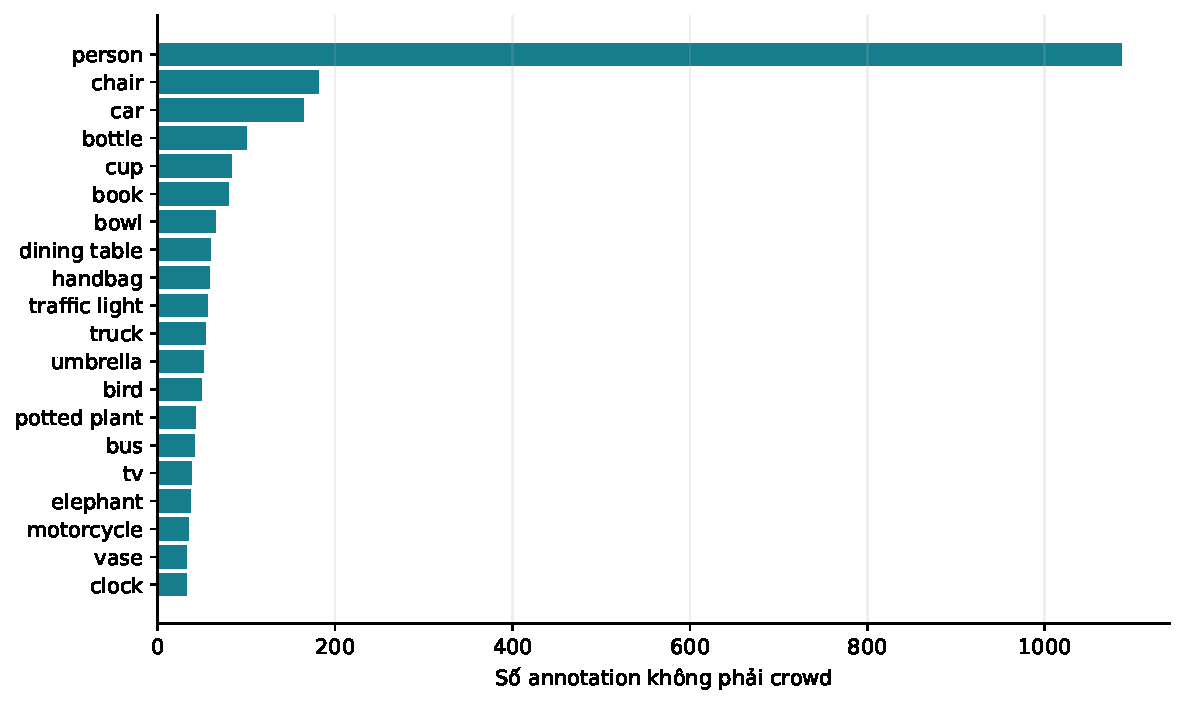
\includegraphics[width=0.94\textwidth]{klygo/distribution.pdf}
\caption{Hai mươi lớp có nhiều annotation không phải crowd nhất trong mẫu. Phân bố được tính trước khi xét dự đoán của mô hình.}
\label{fig:distribution}
\end{figure}
Lớp person có 1.087 annotation, chiếm khoảng 31,3\% trong tổng 3.475 ground truth hợp lệ, trong khi nhiều lớp còn lại có ít mẫu hơn đáng kể. Sự lệch phân bố làm cho P/R/F1 micro chịu ảnh hưởng mạnh từ các lớp phổ biến. AP trung bình theo lớp phân bổ trọng số khác, nên thứ tự mô hình theo một chỉ số không nhất thiết hoàn toàn giống theo chỉ số khác.

Các lớp ít annotation có độ nhạy cao đối với từng dự đoán đúng hoặc sai. Một lớp có AP cao trên vài vật thể không đủ để kết luận mô hình mạnh với lớp đó nói chung. Báo cáo cung cấp số GT theo lớp và bảng đầy đủ ở phụ lục để người đọc đánh giá mức hỗ trợ của mỗi nhận xét. Bộ COCO15 có trong dự án được xem là tài nguyên minh họa và kiểm thử tích hợp, không tham gia vào benchmark chính này.

\section{Môi trường và cấu hình mô hình}
\subsection{Phần cứng và phần mềm}
\begin{table}[H]\centering\small
\caption{Môi trường chạy thực nghiệm}
\begin{tabularx}{\textwidth}{p{5.1cm}Y}
\toprule Thành phần & Giá trị ghi nhận \\\midrule
Hệ điều hành & Windows, build 22631 \\
GPU & NVIDIA GeForce GTX 1650 Ti with Max-Q Design \\
VRAM / RAM hệ thống & Xấp xỉ 4 GiB / 31,73 GiB \\
Python / Klygo & 3.11.9 / 2.1.0 \\
PyTorch / Torchvision & 2.8.0+cu126 / 0.23.0+cu126 \\
CUDA runtime / Ultralytics & 12.6 / 8.3.228 \\
NumPy / Pillow / pycocotools & 2.2.6 / 11.3.0 / 2.0.10 \\
Độ chính xác số / batch & FP32 / 1 \\
Revision source & \code{0ca8a6a77600e1caf770ae8157d2df35360ee719} \\
\bottomrule
\end{tabularx}
\end{table}
CUDA được kiểm tra bằng phép tính tensor thực tế, không chỉ dựa trên việc tìm thấy tên GPU. Các model chạy lần lượt, mỗi lần giữ một model cho suy luận. Yếu tố xung nhịp, nhiệt độ và tải nền của máy không được khóa ở mức hệ điều hành; đây là một giới hạn khi diễn giải chênh lệch thời gian nhỏ.

\subsection{Checkpoint và tham số}
\begin{table}[H]\centering\small
\caption{Cấu hình model và hậu xử lý trong đánh giá chính}
\begin{tabularx}{\textwidth}{p{2.6cm}YY}
\toprule Cấu hình & Trọng số và backend & Tham số đáng chú ý \\\midrule
YOLOv8n & \code{yolov8n.pt}; Ultralytics & imgsz 640; conf 0,001; NMS IoU 0,7; max\_det 100 \\
YOLO-World v2 small & \code{yolov8s-worldv2.pt}; Ultralytics & Như YOLOv8n; vocabulary COCO của checkpoint \\
Faster R-CNN MobileNetV3-Large FPN & \code{COCO\_V1}; Torchvision & min\_size = max\_size = 640; score 0,001; NMS IoU 0,7; tối đa 100 box \\
\bottomrule
\end{tabularx}
\end{table}
Các ngưỡng số giống nhau không bảo đảm tác động giống nhau giữa các mô hình, vì confidence chưa được hiệu chuẩn chung và cấu trúc hậu xử lý khác nhau. Việc đặt min/max size cho Faster R-CNN cũng thay đổi cấu hình mặc định. Mục đích là công bố rõ một cấu hình giới hạn tài nguyên, không tái lập điểm model zoo hoặc chứng minh một họ kiến trúc luôn hơn họ khác.

Không áp dụng thêm một vòng NMS Klygo sau kết quả backend. Box chuyển sang định dạng COCO $xywh$, nhãn chuyển theo tên sang category ID gốc. AP được tính với confidence đầu vào thấp để giữ phần lớn đường cong PR. P/R/F1 được trích riêng tại confidence 0,25 và IoU 0,50, sử dụng quy tắc match/ignore của COCOeval.

\section{Kết quả kiểm thử thư viện}
\begin{table}[H]\centering\small
\caption{Phân bố 360 ca unittest theo nhóm; cột thực hiện bao gồm ca skip}
\begin{tabular}{lrrr}
\toprule
Nhóm & Thực hiện & Đạt & Bỏ qua \\
\midrule
archive & 50 & 50 & 0 \\
config & 24 & 24 & 0 \\
datasets & 34 & 34 & 0 \\
files & 85 & 85 & 0 \\
integration & 4 & 1 & 3 \\
media & 8 & 8 & 0 \\
models & 76 & 72 & 4 \\
outputs & 28 & 28 & 0 \\
postprocessing & 7 & 7 & 0 \\
preprocessing & 12 & 12 & 0 \\
test\_cross\_modules & 1 & 1 & 0 \\
test\_e2e\_zero\_ram & 1 & 1 & 0 \\
test\_path\_conventions & 2 & 2 & 0 \\
test\_public\_api & 4 & 4 & 0 \\
test\_public\_imports & 3 & 3 & 0 \\
utils & 11 & 11 & 0 \\
validators & 6 & 6 & 0 \\
visual & 4 & 4 & 0 \\
\bottomrule
\end{tabular}

\label{tab:tests}
\end{table}
Tổng cộng 353 ca đạt, 7 ca bỏ qua, không có fail hoặc error sau khi đủ phụ thuộc. Ba ca skip thuộc quy trình COCO15 cần dataset và bundle đã sinh; bốn ca opt-in cần đường dẫn checkpoint thật cho YOLO, YOLO-World, Grounding DINO và Locate Anything. Hai mô hình YOLO đã được chạy thật qua mã thực nghiệm báo cáo, nhưng các ca opt-in tương ứng trong unittest vẫn được ghi đúng là skip vì không cấu hình biến môi trường của chúng.

Công cụ audit cả 12 mô-đun cũng hoàn tất với trạng thái đạt đối với source, tài liệu, ví dụ và hợp đồng notebook. Các kiểm tra này hỗ trợ RQ1 và RQ2 ở mức phần mềm. Chúng không chứng minh mọi backend đã chạy trên mọi loại phần cứng, và không suy ra tỷ lệ nhận dạng đúng ngoài dữ liệu đánh giá.

\section{Chất lượng phát hiện trên 500 ảnh}
\subsection{AP tổng hợp và precision--recall}
\begin{table}[H]\centering
\caption{Chất lượng phát hiện sau pipeline Klygo trên cùng 500 ảnh; điểm tính theo phần trăm}
\begin{tabular}{lrrr}
\toprule
Mô hình & AP (\%) & AP50 (\%) & AP75 (\%) \\
\midrule
YOLOv8n & 38{,}24 & 52{,}55 & 41{,}66 \\
YOLO-World & 39{,}07 & 53{,}23 & 42{,}41 \\
Faster R-CNN & 25{,}08 & 39{,}49 & 26{,}31 \\
\bottomrule
\end{tabular}

\label{tab:quality}
\end{table}
YOLO-World có AP cao nhất trong ba cấu hình được đo, hơn YOLOv8n khoảng 0,82 điểm phần trăm. Chênh lệch này nhỏ so với sự khác nhau giữa từng lớp, nên chưa đủ để kết luận ưu thế ổn định trên dữ liệu khác. Faster R-CNN thấp hơn trong cấu hình khảo sát; kết quả gắn với checkpoint MobileNetV3, chính sách resize và ngưỡng cụ thể, không đại diện cho mọi mô hình hai giai đoạn.

AP50 của cả ba đều cao hơn AP75, phù hợp với việc ngưỡng IoU chặt hơn đòi hỏi box chính xác hơn. Điều này gợi ý cần phân tích cả định vị thay vì chỉ nhìn số đối tượng được gán đúng tên. Tuy nhiên, khoảng cách AP50--AP75 không tách riêng hoàn toàn lỗi định vị khỏi các yếu tố khác của đường cong PR, nên không được diễn giải thành tỷ lệ chính xác của một loại lỗi duy nhất.

\begin{figure}[H]\centering
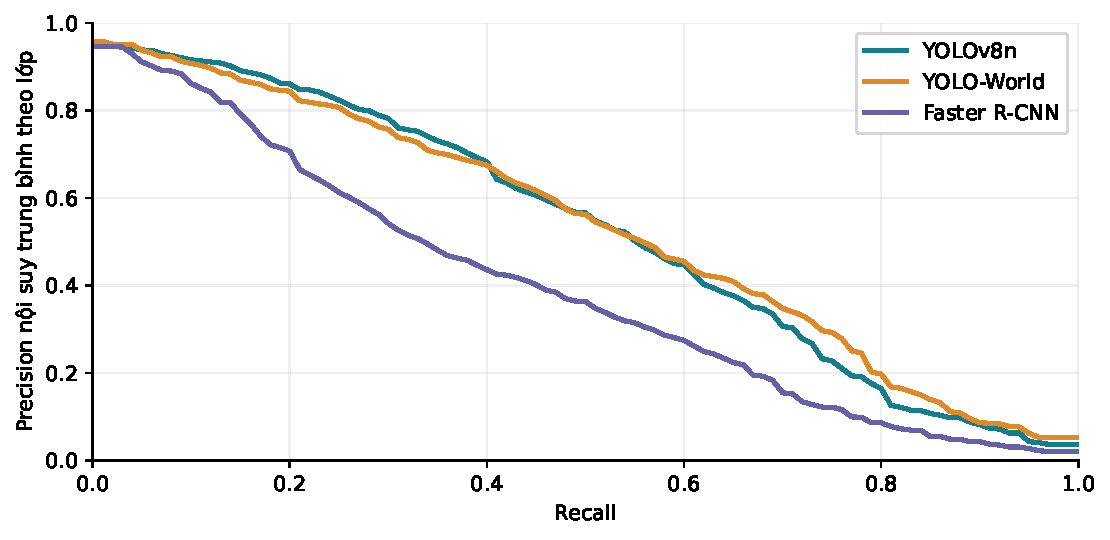
\includegraphics[width=0.94\textwidth]{klygo/pr.pdf}
\caption{Precision nội suy trung bình theo lớp tại IoU 0,50. Đây là đường macro từ COCOeval, khác P/R micro ở một điểm confidence.}
\label{fig:pr}
\end{figure}
Đường cong cho thấy precision giảm khi yêu cầu đạt recall cao hơn. Nó giúp nhìn rộng hơn một điểm confidence 0,25 và thể hiện mức mất precision để tăng độ bao phủ. Phần đuôi đường cong chịu ảnh hưởng số dự đoán tối đa, score threshold, các vật thể khó và khả năng nhận dạng. Do score đã được làm tròn trong builder, các nhóm dự đoán đồng hạng còn có thể tác động đến thứ tự tích lũy; đây là đặc điểm của pipeline đã đánh giá.

\subsection{Điểm làm việc tại confidence 0,25}
\begin{table}[H]\centering\small
\caption{Số đếm và P/R/F1 micro tại confidence 0,25, IoU 0,50}
\begin{tabular}{lrrrrrr}
\toprule
Mô hình & TP & FP & FN & P & R & F1 \\
\midrule
YOLOv8n & 1752 & 695 & 1723 & 0{,}7160 & 0{,}5042 & 0{,}5917 \\
YOLO-World & 1895 & 1003 & 1580 & 0{,}6539 & 0{,}5453 & 0{,}5947 \\
Faster R-CNN & 1574 & 3258 & 1901 & 0{,}3257 & 0{,}4529 & 0{,}3790 \\
\bottomrule
\end{tabular}

\label{tab:operating}
\end{table}
YOLOv8n có Precision khoảng 0,716 và Recall khoảng 0,504. YOLO-World tìm được thêm 143 TP so với YOLOv8n, đồng thời có thêm 308 FP; vì vậy Recall cao hơn nhưng Precision thấp hơn tại cùng ngưỡng. F1 của hai cấu hình gần nhau, khoảng 0,592 và 0,595. Những con số này minh họa vì sao một thay đổi về số TP không thể được đánh giá tách khỏi số FP và FN.

Faster R-CNN tạo nhiều FP hơn tại điểm làm việc đã chọn. Không thể từ đó kết luận confidence 0,25 có cùng ý nghĩa xác suất cho cả ba model. Trong một ứng dụng triển khai, người dùng có thể hiệu chuẩn hoặc chọn ngưỡng theo chi phí lỗi trên một tập phát triển riêng. Báo cáo không thực hiện bước tối ưu đó trên chính tập đánh giá, vì làm như vậy sẽ làm thay đổi cách diễn giải kết quả kiểm chứng.

\subsection{Kết quả theo kích thước vật thể}
\begin{table}[H]\centering
\caption{AP theo các nhóm kích thước của COCOeval}
\begin{tabular}{lrrr}
\toprule
Mô hình & AP small (\%) & AP medium (\%) & AP large (\%) \\
\midrule
YOLOv8n & 21{,}75 & 44{,}43 & 56{,}53 \\
YOLO-World & 26{,}21 & 43{,}44 & 55{,}41 \\
Faster R-CNN & 5{,}51 & 29{,}04 & 51{,}84 \\
\bottomrule
\end{tabular}

\label{tab:sizeap}
\end{table}
Trong mẫu này, nhóm small khó hơn rõ rệt ở cả ba mô hình. YOLO-World có AP small 26,21\%, cao hơn 21,75\% của YOLOv8n, trong khi Faster R-CNN chỉ đạt 5,51\% theo cấu hình giới hạn kích thước đang dùng. Ở nhóm large, khoảng cách giữa các mô hình thu hẹp. Kết quả phù hợp với nhu cầu giữ chi tiết ảnh khi phát hiện vật thể nhỏ, nhưng không đủ xác định riêng resize là nguyên nhân của mọi sai khác.

COCOeval phân nhóm bằng diện tích annotation gốc, không bằng cách tự so kích thước box dự đoán với một ngưỡng pixel sau resize. Một lớp có thể có mặt trong nhóm large mà không có ground truth trong nhóm small. Vì vậy, các AP theo kích thước có thể được trung bình trên các tập lớp hợp lệ khác nhau; chúng cần được xem cùng quy mô dữ liệu, không như ba bài toán có cùng phân bố hoàn toàn.

\subsection{Khác biệt theo lớp}
\begin{table}[H]\centering\small
\caption{AP theo lớp của 12 lớp nhiều GT nhất; các cột mô hình là AP tính bằng phần trăm}
\begin{tabular}{lrrrr}
\toprule
Lớp & GT hợp lệ & YOLOv8n & YOLO-World & Faster R-CNN \\
\midrule
person & 1087 & 51{,}20 & 54{,}55 & 32{,}48 \\
chair & 181 & 29{,}19 & 30{,}86 & 15{,}20 \\
car & 164 & 33{,}08 & 37{,}25 & 17{,}54 \\
bottle & 100 & 31{,}59 & 41{,}43 & 16{,}33 \\
cup & 83 & 41{,}46 & 46{,}58 & 17{,}59 \\
book & 80 & 11{,}84 & 11{,}68 & 2{,}27 \\
bowl & 65 & 40{,}38 & 45{,}70 & 21{,}30 \\
dining table & 59 & 27{,}34 & 27{,}03 & 17{,}91 \\
handbag & 58 & 11{,}14 & 20{,}04 & 3{,}23 \\
traffic light & 56 & 19{,}75 & 15{,}15 & 10{,}49 \\
truck & 54 & 26{,}40 & 28{,}14 & 15{,}53 \\
umbrella & 52 & 46{,}14 & 45{,}67 & 26{,}39 \\
\bottomrule
\end{tabular}

\label{tab:classes}
\end{table}
Các lớp trong bảng được chọn theo số ground truth, không theo việc mô hình nào có điểm cao. Person có AP cao hơn book và handbag đối với cả ba cấu hình. Điều này cho thấy điểm tổng hợp che khuất nhiều khác biệt giữa các nhóm vật thể. Đặc biệt, book có 80 annotation nhưng AP chỉ khoảng 11,8\% đối với hai biến thể YOLO, nên không thể giải thích mọi điểm thấp chỉ bằng thiếu mẫu.

YOLO-World không cao hơn YOLOv8n trên mọi lớp: traffic light, dining table và umbrella trong bảng có các mức chênh lệch khác nhau. Những kết quả này củng cố cách chọn mô hình theo tập lớp và mục tiêu ứng dụng thay vì chỉ lấy một AP tổng hợp. Các lớp ít mẫu và lớp không có GT được giữ trong bảng đầy đủ ở phụ lục, với ký hiệu không áp dụng khi metric không xác định.

\section{Độ trễ và sự đánh đổi chất lượng--thời gian}
\subsection{Thiết kế phép đo}
Một trăm ảnh đầu theo thứ tự manifest được nạp thành ảnh RGB trong RAM. Mỗi model warm-up năm lần, sau đó đo ba lượt trên cùng 100 ảnh. Các nhánh đều batch bằng một, FP32, inference mode và có CUDA synchronize trước/sau timer. Tải mạng, đọc ảnh từ đĩa và nạp checkpoint nằm ngoài vùng đo. Model được đánh giá lần lượt trên một GPU.

\begin{table}[H]\centering
\caption{Thời gian predict trên 100 ảnh, ba lượt; 300 lần gọi mỗi model}
\begin{tabular}{lrrrr}
\toprule
Mô hình & TB (ms) & Trung vị & p90 & FPS tuần tự \\
\midrule
YOLOv8n & 27{,}02 & 28{,}32 & 30{,}92 & 37{,}01 \\
YOLO-World & 32{,}46 & 34{,}13 & 36{,}24 & 30{,}81 \\
Faster R-CNN & 61{,}54 & 55{,}37 & 88{,}47 & 16{,}25 \\
\bottomrule
\end{tabular}

\label{tab:latency}
\end{table}
YOLOv8n có độ trễ trung bình thấp nhất trong cấu hình đo. YOLO-World mất thêm khoảng 5,44 ms nhưng có AP cao hơn khoảng 0,82 điểm phần trăm trên mẫu chất lượng. Faster R-CNN chậm hơn và có điểm thấp hơn trong lần khảo sát này. Các so sánh chỉ phản ánh cấu hình end-to-end qua Klygo; chúng không tách độc lập đóng góp của backbone, backend, preprocessing và output conversion.

\begin{figure}[H]\centering
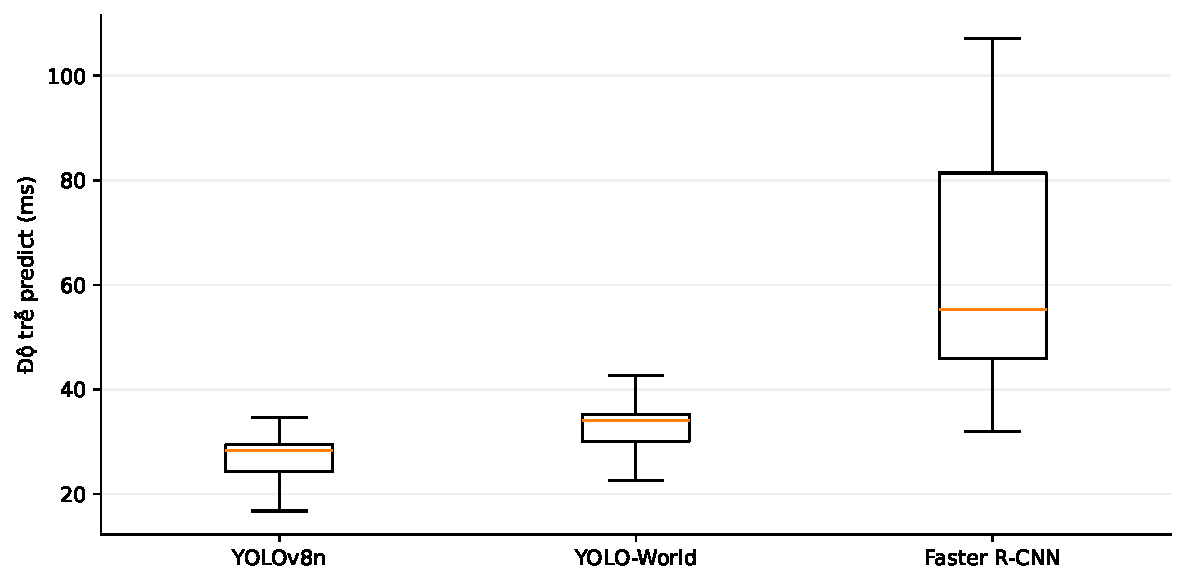
\includegraphics[width=0.94\textwidth]{klygo/latency.pdf}
\caption{Phân bố độ trễ predict qua 300 lần gọi mỗi model. Boxplot lược điểm ngoại lai khi vẽ; tệp latency vẫn giữ toàn bộ mẫu.}
\label{fig:latency}
\end{figure}
Trung vị Faster R-CNN thấp hơn trung bình và p90 lớn hơn đáng kể, cho thấy thời gian không có phân bố đối xứng đơn giản. Sự khác biệt kích thước/tỷ lệ ảnh, số box và công việc hậu xử lý có thể cùng góp phần vào biến thiên. Đề tài chưa thực hiện phân rã timer theo từng thành phần nên không gán một nguyên nhân duy nhất cho các lần gọi chậm.

\begin{table}[H]\centering
\caption{Độ trễ predict trung bình theo từng lượt lặp}
\begin{tabular}{lrrr}
\toprule
Mô hình & Lượt 1 (ms) & Lượt 2 (ms) & Lượt 3 (ms) \\
\midrule
YOLOv8n & 27{,}51 & 27{,}14 & 26{,}40 \\
YOLO-World & 33{,}09 & 31{,}96 & 32{,}32 \\
Faster R-CNN & 61{,}81 & 61{,}29 & 61{,}52 \\
\bottomrule
\end{tabular}

\end{table}
Các lượt dùng lại cùng ảnh, nên có thể phản ánh biến thiên do tải máy, cache hoặc xung nhịp. Ba lượt không biến 100 ảnh thành 300 ảnh độc lập để đánh giá tổng quát hóa. FPS trong Bảng~\ref{tab:latency} được suy từ thời gian trung bình tuần tự, không phải tốc độ tối đa của hệ thống xử lý video có pipeline hoặc batching.

\begin{figure}[H]\centering
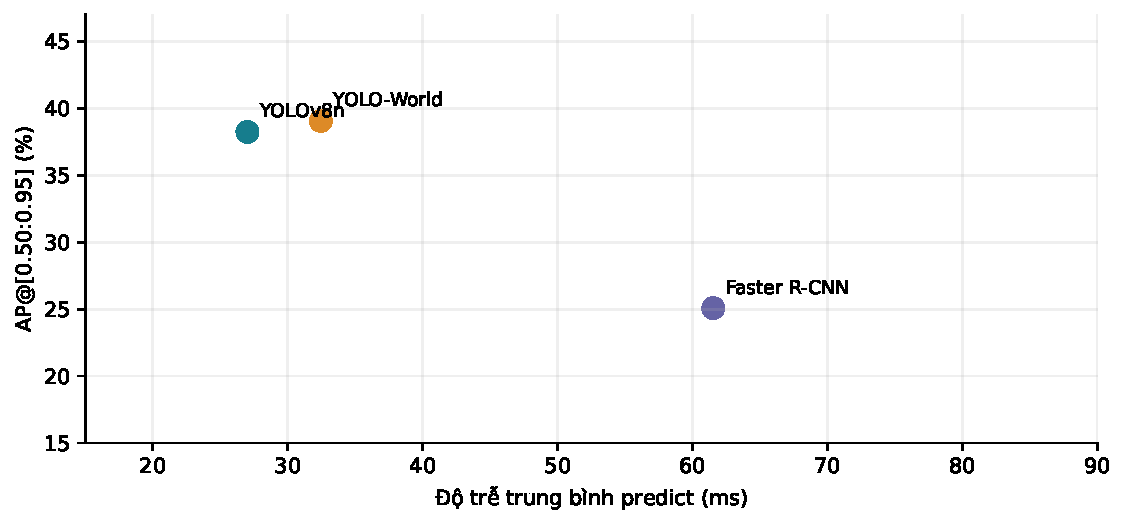
\includegraphics[width=0.94\textwidth]{klygo/tradeoff.pdf}
\caption{Chất lượng trên 500 ảnh và độ trễ lặp trên 100 ảnh. Mỗi điểm biểu diễn một cấu hình hệ thống, không phải một phép đo riêng của backend.}
\label{fig:tradeoff}
\end{figure}

\subsection{Chi phí của lớp điều phối predict}
Để trả lời RQ4, mã gọi cùng model theo hai cách: trực tiếp \code{forward([image])} trả frame \code{Detection}, và \code{predict(image)} tạo kết quả có điều phối nguồn, cấu hình, metadata và collection. Cả hai giữ preprocessing, inference, hậu xử lý backend và đóng gói Detection. Vì baseline vẫn sử dụng adapter và kiểu đầu ra Klygo, phép đo chỉ tách chi phí lifecycle của predict; nó không đo toàn bộ chi phí Klygo so với một framework thuần.

\begin{table}[H]\centering\small
\caption{Đo cặp predict và forward với cùng inference mode và đầu ra tương đương}
\begin{tabular}{lrrrr}
\toprule
Mô hình & forward (ms) & predict (ms) & $\Delta$ (ms) & $\Delta$ (\%) \\
\midrule
YOLOv8n & 24{,}53 & 27{,}02 & 2{,}49 & 10{,}15 \\
YOLO-World & 29{,}98 & 32{,}46 & 2{,}48 & 8{,}28 \\
Faster R-CNN & 59{,}16 & 61{,}54 & 2{,}38 & 4{,}03 \\
\bottomrule
\end{tabular}

\label{tab:overhead}
\end{table}
Mỗi mô hình có 300 cặp đo, đổi thứ tự nhánh theo ảnh và lượt. Không có cặp nào khác về số box, nhãn, tọa độ hoặc score vượt sai số cho phép. Chênh lệch trung bình khoảng 2,38--2,49 ms, tương ứng khoảng 4,03--10,15\% của baseline forward. Tỷ lệ tương đối của YOLOv8n lớn hơn vì thời gian nền của nó thấp hơn; không có nghĩa lớp điều phối phải thực hiện một lượng công việc gấp đôi cho model đó.

\begin{figure}[H]\centering
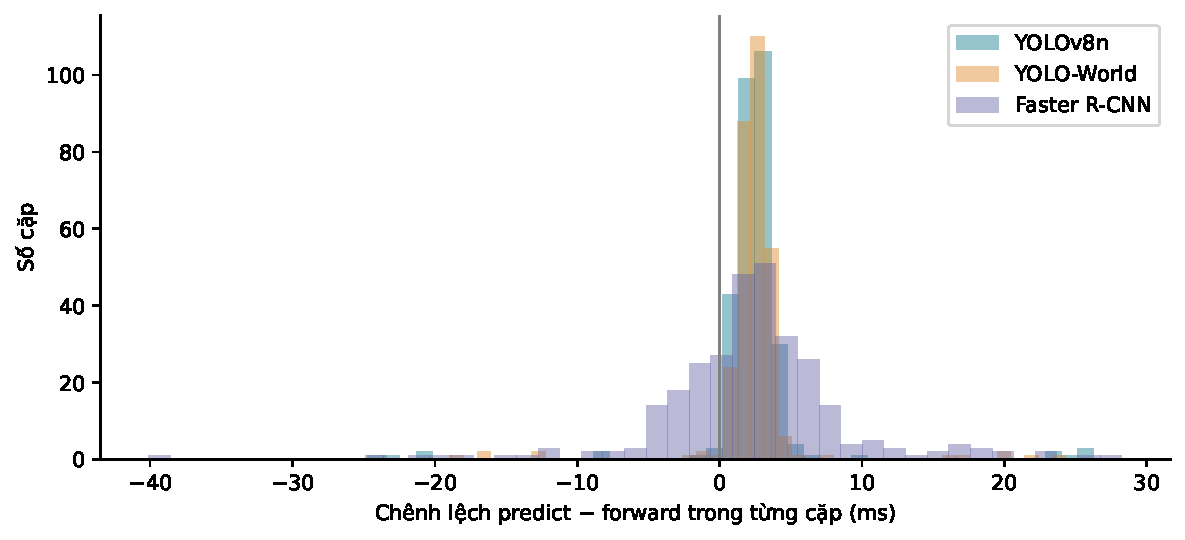
\includegraphics[width=0.94\textwidth]{klygo/overhead.pdf}
\caption{Phân bố chênh lệch trong từng cặp thời gian. Chênh lệch âm riêng lẻ được giữ lại như biến thiên đo, không bị cắt về không.}
\end{figure}
Các cặp chậm hoặc chênh lệch âm có thể xuất hiện vì hai lời gọi không chạy tại cùng một thời điểm tuyệt đối. Vì thế, chênh lệch không nên được xem là hằng số chính xác của mọi lần gọi. Kết quả hỗ trợ một nhận xét có phạm vi: trên nguồn PIL đã sẵn trong RAM và batch một, lớp điều phối bổ sung vài mili giây trong ba cấu hình được đo. Tình huống video, ảnh lazy chưa giải mã, batch lớn hoặc nhiều luồng cần đo lại.

\section{Phân tích trường hợp thành công và lỗi}
Ba ảnh được chọn bằng quy tắc công bố: ảnh tốt có F1 YOLOv8n cao nhất trong nhóm ít nhất ba GT hợp lệ; ảnh khó có tổng FP+FN YOLOv8n lớn nhất trong cùng nhóm; ảnh small có nhiều annotation small nhất sau khi loại hai ảnh trước. Tiêu chí sử dụng YOLOv8n làm điểm chọn ảnh, nên đây là phân tích trường hợp có chủ đích, không phải một ước lượng trung lập về phân bố lỗi của toàn bộ mô hình.

Ảnh ID 67406 có bốn ground truth hợp lệ. Hai mô hình YOLO đều đạt bốn TP, không FP tại điểm làm việc; Faster R-CNN có bốn TP nhưng thêm sáu FP. Trường hợp này cho thấy việc tìm đủ vật thể vẫn có thể đi kèm kết quả dư thừa. Ảnh ID 65288 là một cảnh có nhiều đối tượng, che khuất và khác biệt tỷ lệ: 37 GT hợp lệ nhưng chỉ có 6, 10 và 6 TP tương ứng. Ảnh ID 432898 có 35 GT hợp lệ và nhiều vật thể nhỏ; Faster R-CNN có 11 TP nhưng 46 FP tại ngưỡng đã chọn.

\begin{figure}[H]\centering\includegraphics[width=\textwidth]{klygo/case_good.png}
\caption[So sánh kết quả trên ảnh COCO ID 67406]{Ảnh COCO ID 67406; tiêu chí chọn: F1 cao nhất của YOLOv8n trong các ảnh có ít nhất ba GT hợp lệ. Dự đoán hiển thị tại confidence 0,25; chỉ vẽ tối đa 20 box và lược nhãn trên ảnh để tránh che khuất. Số box trong tiêu đề là số trước giới hạn hiển thị. Metric dùng toàn bộ dự đoán theo cấu hình.}\label{fig:case-good}
\end{figure}

\begin{figure}[H]\centering\includegraphics[width=\textwidth]{klygo/case_hard.png}
\caption[So sánh kết quả trên ảnh COCO ID 65288]{Ảnh COCO ID 65288; tiêu chí chọn: tổng FP và FN lớn nhất của YOLOv8n trong các ảnh có ít nhất ba GT hợp lệ. Dự đoán hiển thị tại confidence 0,25; chỉ vẽ tối đa 20 box và lược nhãn trên ảnh để tránh che khuất. Số box trong tiêu đề là số trước giới hạn hiển thị. Metric dùng toàn bộ dự đoán theo cấu hình.}\label{fig:case-hard}
\end{figure}

\begin{figure}[H]\centering\includegraphics[width=\textwidth]{klygo/case_small.png}
\caption[So sánh kết quả trên ảnh COCO ID 432898]{Ảnh COCO ID 432898; tiêu chí chọn: số annotation small nhiều nhất, sau khi loại hai ảnh đã chọn. Dự đoán hiển thị tại confidence 0,25; chỉ vẽ tối đa 20 box và lược nhãn trên ảnh để tránh che khuất. Số box trong tiêu đề là số trước giới hạn hiển thị. Metric dùng toàn bộ dự đoán theo cấu hình.}\label{fig:case-small}
\end{figure}

Các panel giữ vị trí ảnh giống nhau giữa ground truth và model. Để hình không bị che bởi nhãn chồng lấn, chỉ vẽ tối đa 20 box và không in nhãn lên từng box trong montage. Dữ liệu định lượng sử dụng toàn bộ dự đoán đã lưu. Một box dự đoán có vẻ nằm gần vật thể khi nhìn ảnh vẫn có thể là FP nếu không đúng lớp hoặc chưa đạt IoU 0,50; các số đếm được xác định bằng quy tắc ghép, không bằng nhận xét bằng mắt.

Từ ba trường hợp có thể đặt ra hướng khảo sát tiếp theo: kiểm tra ảnh dày vật thể và che khuất, tăng độ phân giải cho nhóm small, hoặc điều chỉnh ngưỡng theo yêu cầu giảm FP trên một tập phát triển riêng. Những hướng này là giả thuyết cần thử nghiệm thêm; số liệu hiện tại chưa đủ chứng minh một thay đổi cụ thể sẽ cải thiện đồng thời mọi chỉ số.

\section{Giới hạn và các mối đe dọa tới tính hợp lệ}
\textbf{Giới hạn về dữ liệu.} Mẫu 500 ảnh chỉ là một phần validation. Các lớp hiếm có số mẫu thấp và một lớp không có GT hợp lệ, làm điểm theo lớp không ổn định. Các checkpoint được huấn luyện hoặc tiền huấn luyện trên các dữ liệu do tác giả công bố; báo cáo không chứng minh toàn bộ dữ liệu tiền huấn luyện độc lập với mọi ảnh/khái niệm trong mẫu. Do đó không dùng kết quả này để khẳng định zero-shot trên lớp mới.

\textbf{Giới hạn về cấu hình.} Các model dùng chính sách resize khác nhau, score chưa được hiệu chuẩn chung và Faster R-CNN đã thay đổi min/max size so với mặc định. Kết quả là so sánh các cấu hình triển khai cụ thể. Builder Klygo làm tròn dữ liệu, nên AP có thể khác kết quả tính từ tensor gốc. Thí nghiệm chưa đo riêng ảnh hưởng của làm tròn hoặc resize.

\textbf{Giới hạn về hiệu năng.} Chỉ dùng một máy và một GPU, không khóa xung nhịp, nhiệt độ hoặc tải nền. Thời gian không bao gồm mạng, đọc đĩa, hiển thị và nạp checkpoint. Độ trễ thấp trong phép đo không chứng minh hệ thống phục vụ thời gian thực cho một ứng dụng có thêm nhiều bước khác.

\textbf{Giới hạn về suy luận thống kê.} Báo cáo công bố điểm và các lượt lặp thời gian, chưa cung cấp khoảng tin cậy bootstrap cho chênh lệch AP. Chênh lệch 0,82 điểm phần trăm giữa hai biến thể YOLO vì vậy được xem là kết quả quan sát trên mẫu cố định, không phải khẳng định có ý nghĩa thống kê. Tính tương đương của hai nhánh thời gian được kiểm tra trên dữ liệu đo, không phải chứng minh cho mọi đầu vào có thể có.

\textbf{Giới hạn về phạm vi sản phẩm.} Kiểm thử giả lập không thay thế checkpoint thật; khả năng có mã adapter không đồng nghĩa mọi backend đã được xác nhận trong báo cáo. Grounding DINO, Locate Anything và KerasHub chưa tham gia phép đo chính. Khả năng streaming có kiểm thử hợp đồng, nhưng chưa có benchmark bộ nhớ dài hạn hay thử tải nhiều người dùng.

\section{Thực nghiệm mining và kiểm chứng dữ liệu xuất}
\label{sec:mining-exp}
Thực nghiệm mở rộng dùng revision \code{c4388f1}. Từ thứ tự 500 ID đã cố định trong manifest, 300 ảnh đầu làm tập tuyển chọn/train, 100 ảnh tiếp theo làm validation và 100 ảnh cuối làm test. Đây là phép chia phục vụ nghiên cứu nhỏ trên COCO val2017, không phải tập train/test chính thức của COCO. Các số AP của ba checkpoint ở phần trước vẫn được tính trên đủ 500 ảnh với checkpoint chưa fine-tune; các checkpoint fine-tune không được đánh giá lại trên những ảnh đã dùng train để báo kết quả tổng quát hóa.

Mining chỉ truy cập tập train. Annotation crowd bị loại khỏi bộ YOLO của thí nghiệm; box được chặn trong biên ảnh và chỉ giữ diện tích dương. Tập tuyển chọn có 300 ảnh và 2.099 box. Ba tập được tách bằng ID ảnh; nghiên cứu chưa bổ sung loại trùng ngữ nghĩa hoặc nhóm ảnh gần giống giữa các split. Không sử dụng nhãn tự động.

Random, Weighted, Diversity và Rare-first có ngân sách 150 ảnh. Diversity dùng 150 cụm và chọn một đại diện mỗi cụm; seed chọn bằng 42. Quality dùng ngưỡng 0,5; Boxes yêu cầu ít nhất hai box; Class yêu cầu có lớp person; Quota và Coverage đặt quota ba ảnh/lớp với giới hạn 150; Balance dùng median theo số ảnh chứa lớp. Các bộ lọc và quota có thể trả ít hơn giới hạn nên không được xem là đối chứng cùng ngân sách cho mọi hàng.

Thời gian chọn lấy trung vị ba lần sau một lượt warm-up trên collection đã nạp, chạy CPU. Weighted và Diversity bao gồm tính điểm hoặc trích đặc trưng/phân cụm trong mỗi lần đo; không dùng báo cáo tính sẵn để che chi phí chuẩn bị. Thời gian không gồm export. Hàng full chỉ tham chiếu collection đầu vào nên thời gian gần bằng không, không phải chi phí đọc dữ liệu từ đĩa.

\begin{table}[H]\centering\small
\caption{Benchmark tuyển chọn trên 300 ảnh; IR chỉ tính các lớp hiện diện}
\begin{tabular}{lrrrrr}
\toprule
Cách chọn & Ảnh & Box & Lớp & IR & Chọn (ms) \\
\midrule
full & 300 & 2099 & 77 & 167.0 & 0.0 \\
random & 150 & 1070 & 76 & 79.0 & 9.3 \\
weighted & 150 & 1410 & 77 & 69.0 & 4693.7 \\
diversity & 150 & 1172 & 75 & 87.0 & 5980.4 \\
rare-first & 150 & 904 & 76 & 42.0 & 4337.5 \\
coverage & 97 & 835 & 77 & 45.0 & 130.2 \\
quota & 97 & 835 & 77 & 45.0 & 93.7 \\
quality & 150 & 1160 & 74 & 91.0 & 4374.7 \\
boxes & 150 & 1266 & 74 & 92.0 & 10.0 \\
class & 150 & 1321 & 69 & 150.0 & 9.2 \\
balance & 212 & 1553 & 77 & 111.0 & 141.0 \\
\bottomrule
\end{tabular}

\end{table}
Quota và Coverage tạo cùng tập ảnh do đi qua cùng hàm greedy; chênh lệch thời gian đo không phải bằng chứng khác biệt thuật toán. Balance có thể giữ hơn 150 ảnh và không bị áp cùng ngân sách. Weighted giữ nhiều box hơn Random dù số ảnh bằng nhau, nên thực nghiệm huấn luyện cùng số ảnh chưa phải cùng số đối tượng được quan sát. Khi đánh giá hiệu quả chọn cần công bố cả hai đơn vị.

\begin{figure}[H]\centering
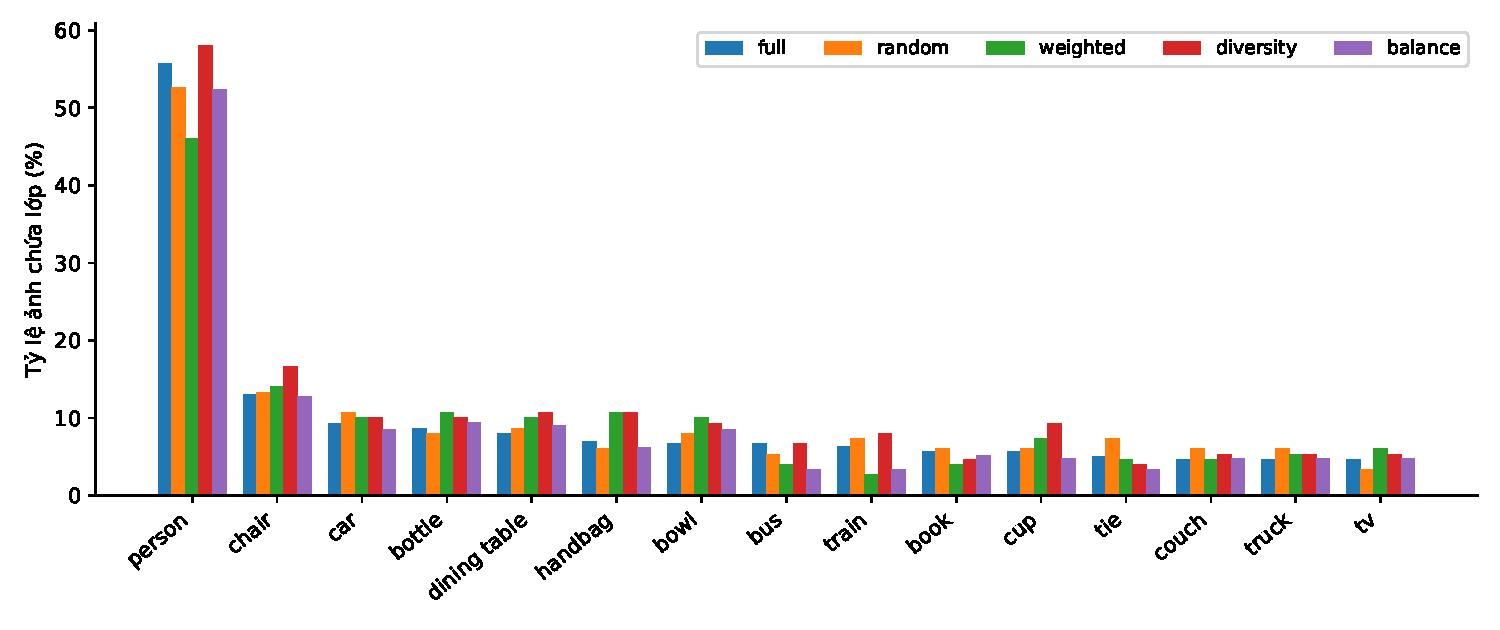
\includegraphics[width=\textwidth]{klygo/mining_distribution.pdf}
\caption{Phân bố 15 lớp phổ biến nhất của tập đầu vào, chuẩn hóa theo số ảnh của từng tập}
\end{figure}
\begin{figure}[H]\centering
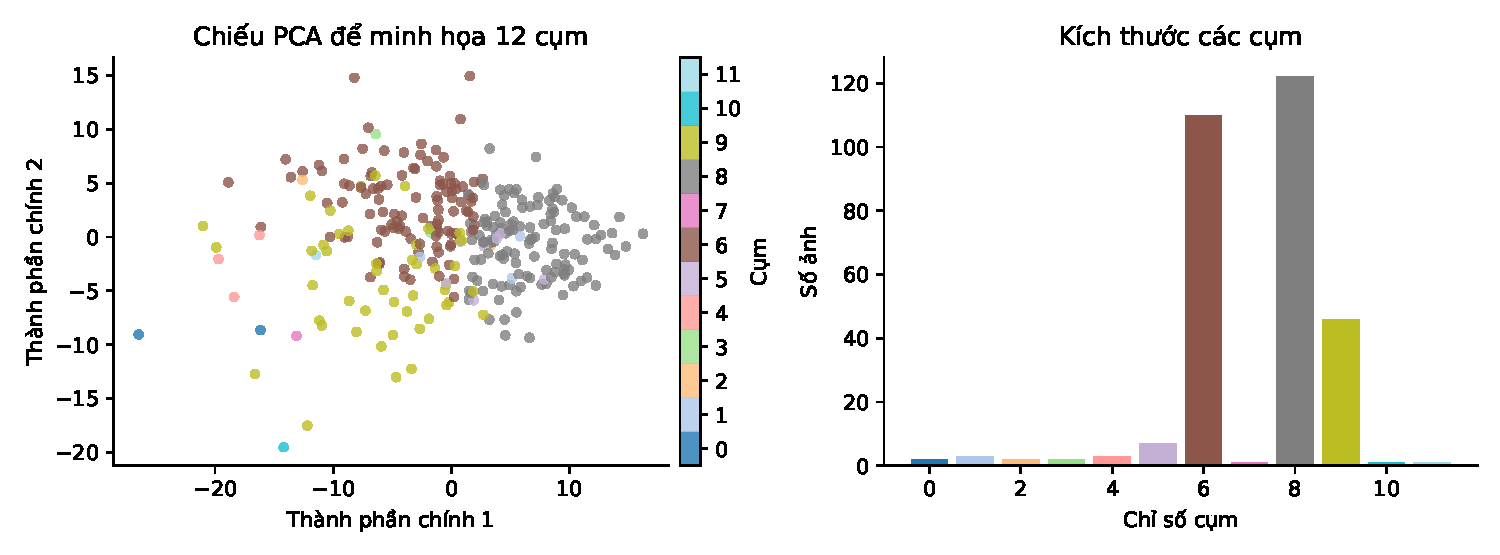
\includegraphics[width=\textwidth]{klygo/mining_clusters.pdf}
\caption{Minh họa 12 cụm trên 300 ảnh; PCA chỉ dùng để vẽ, không dùng để chọn mẫu}
\end{figure}
Hình phân cụm dùng $K=12$ để quan sát và được lưu riêng với cấu hình tuyển chọn $K=150$. Phân tích thành phần chính (PCA) chiếu dữ liệu lên hai hướng có phương sai lớn để minh họa. Khoảng cách trên mặt phẳng này không bảo toàn toàn bộ khoảng cách 726 chiều; ảnh gần nhau trên hình chưa đủ để kết luận là ảnh trùng. Không lựa chọn $K$ hay trọng số dựa trên điểm test.

\subsection{Từ export annotation đến bộ dữ liệu huấn luyện}
Trong revision này, \code{Detections.export(format="yolo")} ghi nhãn, registry lớp và manifest, không sao chép ảnh nguồn. Script thực nghiệm ghép ảnh theo \code{source\_path}, đổi tên tương ứng \code{label\_file}, rồi tạo YAML với đường dẫn train/val/test. Việc ghép ảnh và tạo YAML là bước chuẩn bị bổ sung của thực nghiệm, không được quy cho API export tự thực hiện.

Mỗi phương pháp được kiểm tra số ID duy nhất, tập ID là tập con của train, số ảnh/box và số box theo từng lớp sau khi đọc lại bằng \code{datasets.load}. Các kiểm tra đều đạt; nội dung đầu vào được đối chiếu trước và sau mining để xác nhận không bị thay đổi. Kiểm tra round-trip này xác nhận tính toàn vẹn cấu trúc và số nhãn, không thay thế đánh giá chất lượng annotation.

Export đánh lại class ID liên tục theo registry hiện diện của từng tập. Vì các tập có thể thiếu những lớp khác nhau, bộ nhãn được ánh xạ lại theo tên về cùng thứ tự 80 lớp COCO trước khi train. Script \code{prepare\_training\_canonical.py} kiểm tra bảo toàn số box theo tên lớp sau phép đổi ID. Lượt thử trước khi phát hiện khác biệt registry đã được dừng và giữ riêng; chỉ kết quả trong \code{training\_canonical} được dùng ở bảng và biểu đồ huấn luyện.

\section{Fine-tune trên dữ liệu được tuyển chọn}
\label{sec:mining-train}
Bốn cấu hình train là Full (300 ảnh), Random, Weighted và Diversity (mỗi tập 150 ảnh). Mọi lượt bắt đầu từ cùng checkpoint YOLOv8n COCO pretrained. Mỗi cấu hình chạy năm epoch với ba seed huấn luyện 42, 43 và 44; tập được chọn giữ nguyên seed 42. Độ lệch chuẩn vì vậy mô tả biến thiên huấn luyện có điều kiện trên các tập đã cố định, chưa bao gồm biến thiên khi chọn lại dữ liệu.

Vocabulary của model và YAML được giữ đủ 80 lớp để đầu ra có ý nghĩa nhất quán và sử dụng nguyên checkpoint khởi tạo. Tập full train có 77 lớp hiện diện; số lớp có ground truth trong test là 73. Các lớp ít mẫu khiến AP nhạy với một vài dự đoán; không diễn giải trung bình trên tập test nhỏ như mức chất lượng của toàn bộ COCO.

Thiết lập gồm kích thước 320, batch tám, FP32, AdamW, learning rate đầu 0,001, hệ số cuối 0,1, không warm-up, không mosaic/mixup và không early stopping. Số worker đọc dữ liệu bằng không. Sử dụng checkpoint epoch cuối, không chọn checkpoint theo tập test. Chất lượng được đo bằng metric bbox của Ultralytics trên 100 ảnh test, confidence 0,001, NMS IoU 0,7, max detections 100. Quy trình huấn luyện và tham số được lưu kèm \citep{ultralyticsTrain}; phiên bản thực thi được khóa ở 8.3.228. AP ở mục này không trộn với kết quả COCOeval 500 ảnh/kích thước 640 ở phần trước.

\begin{table}[H]\centering\small
\caption{Fine-tune năm epoch: trung bình và độ lệch chuẩn mẫu qua ba seed}
\begin{tabular}{lrrrr}
\toprule
Tập train & Ảnh & AP (\%) & AP50 (\%) & Train (s) \\
\midrule
full & 300 & 10.38 $\pm$ 1.91 & 17.28 & 52.4 \\
random & 150 & 10.10 $\pm$ 0.61 & 16.20 & 30.4 \\
weighted & 150 & 10.38 $\pm$ 0.55 & 16.83 & 30.7 \\
diversity & 150 & 8.00 $\pm$ 1.85 & 14.14 & 30.6 \\
\bottomrule
\end{tabular}

\end{table}
\begin{figure}[H]\centering
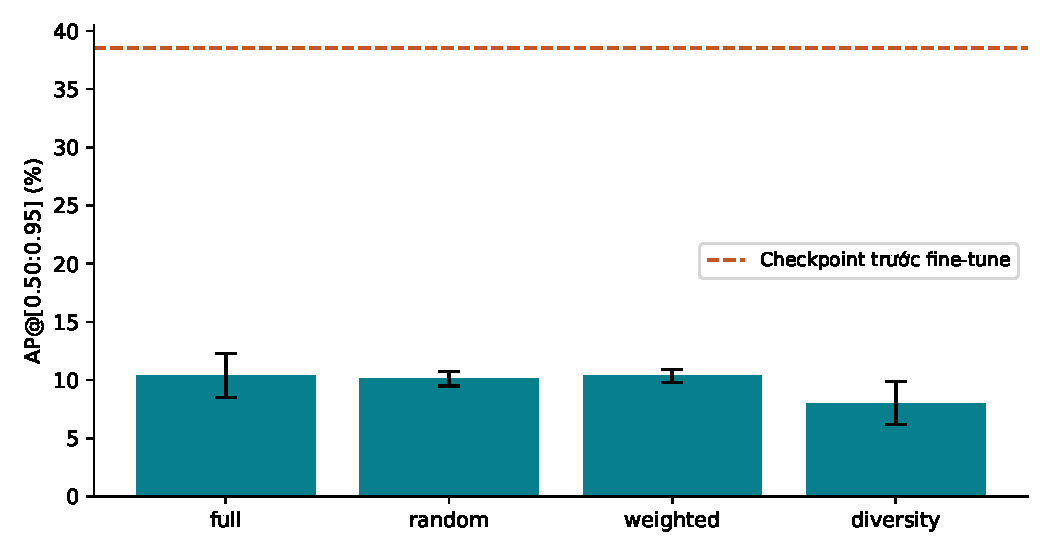
\includegraphics[width=.88\textwidth]{klygo/mining_training.pdf}
\caption{Chất lượng sau fine-tune và checkpoint ban đầu trên cùng tập test}
\end{figure}
Checkpoint ban đầu đạt AP 38.52\% trên cùng 100 ảnh test ở kích thước 320. Weighted chênh +0.28 điểm phần trăm AP so với Random cùng 150 ảnh. Diversity chênh -2.10 điểm phần trăm AP so với Random cùng 150 ảnh. Các chênh lệch là mô tả mẫu; ba seed không đủ để khẳng định khác biệt có ý nghĩa thống kê hoặc ưu thế trên các tập dữ liệu khác. Độ lệch chuẩn phản ánh biến thiên huấn luyện, không phải khoảng tin cậy do lấy mẫu ảnh test.

Thời gian train là thời gian tường của lời gọi train, gồm khởi tạo trainer, lưu checkpoint và xử lý validation bên trong thư viện, không gồm đánh giá test riêng. Đây là so sánh cùng epoch: full có khoảng gấp đôi số batch cập nhật so với mỗi tập con. Chi phí mining cũng cần cộng vào khi xét tổng thời gian. Năm epoch và 100 ảnh test là một thực nghiệm thăm dò; không đủ để xếp hạng phương pháp trên toàn COCO hay suy ra kết quả học từ đầu. Fine-tune ngắn có thể giảm AP so với checkpoint ban đầu do tập nhỏ và thay đổi phân bố; kết quả giảm vẫn được báo cáo.

\section{Benchmark framework gốc và các chế độ Klygo}
\label{sec:execution-exp}
Thực nghiệm dùng YOLOv8n và YOLO-World v2 small ở revision \code{c4388f1}, theo sáu cấu hình đã phân biệt ở Hình~\ref{fig:execution-paths} và bảng tương ứng trong chương thiết kế. Cả sáu nhánh được đo lại trong phiên ngày 07/11/2026; không ghép một hàng mới vào kết quả năm nhánh của phiên trước. Mỗi cặp model/chế độ được nạp trong tiến trình riêng. Đầu vào là cùng 100 ảnh JPEG theo thứ tự manifest, đặt tên để thứ tự duyệt thư mục được xác định. Mỗi nhánh có một lượt warm-up toàn tập rồi ba lượt đo toàn tập; batch một, FP32, kích thước 640, confidence 0,25, IoU 0,7 và max detections 100. Không thay vocabulary YOLO-World.

Lượt thăm dò ở confidence 0,001 dừng tại Klygo native do backend trả box có chiều rộng hoặc chiều cao bằng không, bị validator từ chối. Log và các kết quả Raw của lượt này được giữ riêng, không ghép vào bảng. Benchmark đầy đủ được chạy lại ở confidence 0,25 cho tất cả các nhánh, không loại ảnh gây lỗi. Đây là cấu hình phục vụ suy luận thông thường; chưa chứng minh revision mới hoạt động với mọi box ở ngưỡng rất thấp. Không dùng bảng thời gian này làm thời gian tính AP ở confidence 0,001.

Timer bao gồm giải mã nguồn, suy luận, hậu xử lý và trả kết quả công khai; không gồm nạp trọng số. Với stream, timer kéo dài đến khi tiêu thụ hết iterator. Thời điểm kết quả đầu tiên được quan sát từ phía người gọi, nên ở non-stream/native nó bao gồm chờ hoàn thành collection; không được gọi là độ trễ suy luận của một frame. CUDA được đồng bộ tại ranh giới đo và khi nhận kết quả đầu. Việc chuẩn hóa dự đoán để đối chiếu được thực hiện trong một lượt riêng, ngoài timer.

RAM là RSS đỉnh được lấy mẫu mỗi 10 ms trong tiến trình; VRAM là đỉnh bộ nhớ tensor do PyTorch cấp phát, không phải toàn bộ bộ nhớ thiết bị do trình điều khiển báo. Các cột bộ nhớ là MiB tuyệt đối và có bao gồm model/runtime. Số liệu là trung vị ba lượt. Chênh lệch bộ nhớ so với trước mỗi lượt cũng được lưu trong JSON; phép đo ngắn chưa kiểm chứng giới hạn bộ nhớ của một video kéo dài.

\begin{table}[H]\centering\small
\caption{YOLOv8n: cùng 100 ảnh, các chế độ thực thi}
\begin{tabular}{lrrrrr}
\toprule
Chế độ & Giây & Ảnh/s & Đầu (ms) & RAM & VRAM \\
\midrule
raw & 1.93 & 51.91 & 1926.5 & 1164 & 46 \\
raw stream & 2.14 & 46.77 & 23.7 & 1075 & 46 \\
native & 2.24 & 44.74 & 2235.0 & 1137 & 46 \\
native backend stream & 1.99 & 50.23 & 1990.8 & 1071 & 46 \\
managed & 1.83 & 54.70 & 1828.2 & 1062 & 38 \\
managed stream & 1.99 & 50.26 & 35.1 & 1060 & 38 \\
\bottomrule
\end{tabular}

\end{table}
\begin{table}[H]\centering\small
\caption{YOLO-World: cùng 100 ảnh, các chế độ thực thi}
\begin{tabular}{lrrrrr}
\toprule
Chế độ & Giây & Ảnh/s & Đầu (ms) & RAM & VRAM \\
\midrule
raw & 2.84 & 35.25 & 2836.5 & 1253 & 137 \\
raw stream & 2.60 & 38.47 & 27.2 & 1171 & 137 \\
native & 3.25 & 30.77 & 3250.2 & 1201 & 137 \\
native backend stream & 2.99 & 33.40 & 2994.0 & 1121 & 137 \\
managed & 2.52 & 39.71 & 2518.2 & 1125 & 128 \\
managed stream & 2.54 & 39.33 & 41.9 & 1126 & 128 \\
\bottomrule
\end{tabular}

\end{table}
\begin{figure}[H]\centering
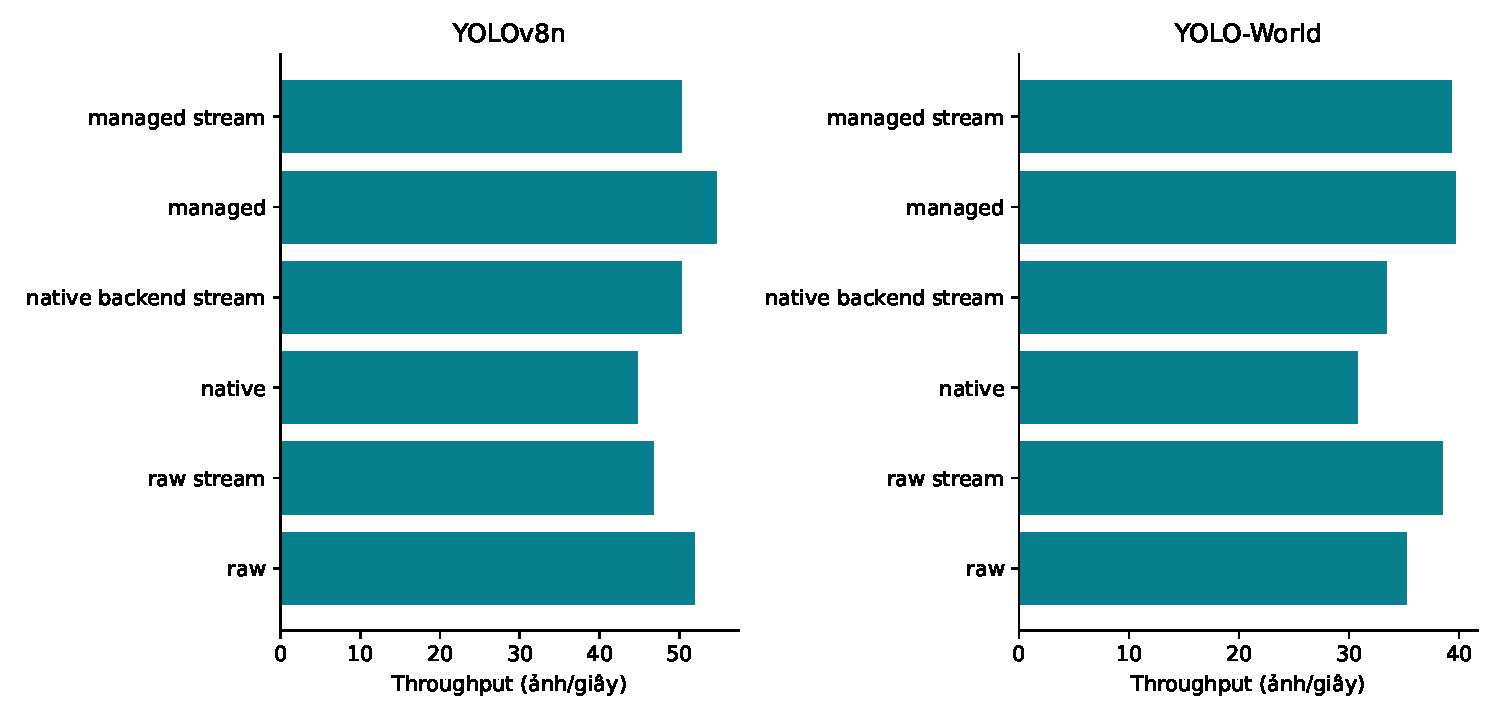
\includegraphics[width=\textwidth]{klygo/execution_throughput.pdf}
\caption{Throughput của framework gốc và các đường thực thi Klygo}
\end{figure}
YOLOv8n: chênh lệch thời gian toàn tập so với Raw là native +16.0\%, native backend stream +3.3\%, managed -5.1\%, managed stream +3.3\%. Dấu dương biểu thị chậm hơn, dấu âm biểu thị nhanh hơn trong phép đo này.

Đối chiếu YOLOv8n có 0/500 cặp frame vượt tiêu chí tương đương: cùng số box, class và sai số tọa độ không quá 0,01 pixel, score không quá 0,001. Sai số lớn nhất theo cách ghép class/score là 0.000000 pixel và 0.000000 điểm score. Phép kiểm tra này dùng dự đoán framework làm tham chiếu, không gọi đó là ground truth.

YOLO-World: chênh lệch thời gian toàn tập so với Raw là native +14.6\%, native backend stream +5.5\%, managed -11.2\%, managed stream -10.4\%. Dấu dương biểu thị chậm hơn, dấu âm biểu thị nhanh hơn trong phép đo này.

Đối chiếu YOLO-World có 0/500 cặp frame vượt tiêu chí tương đương: cùng số box, class và sai số tọa độ không quá 0,01 pixel, score không quá 0,001. Sai số lớn nhất theo cách ghép class/score là 0.000000 pixel và 0.000000 điểm score. Phép kiểm tra này dùng dự đoán framework làm tham chiếu, không gọi đó là ground truth.

Raw trả kiểu dữ liệu của framework, còn Klygo bổ sung container, identity và metadata. Vì đầu ra có chức năng khác nhau, chênh lệch Raw--Klygo là chi phí hoặc lợi ích của đường xử lý hoàn chỉnh, không cô lập thời gian kernel mạng. Native--Managed giúp quan sát thêm ảnh hưởng điều phối nguồn. Không dùng phép đo này để tuyên bố kiến trúc mạng đã được tối ưu, hoặc mọi cấu hình stream đều nhanh hơn non-stream.

Các chế độ được chạy nối tiếp trong những tiến trình khác nhau, chưa hoán đổi thứ tự theo một thiết kế ngẫu nhiên cân bằng. Tải hệ điều hành, cache đĩa và trạng thái nhiệt/xung GPU vẫn có thể tạo nhiễu; ba lượt đo không loại bỏ được các yếu tố đó. Những chênh lệch nhỏ cần được kiểm tra lại trên nhiều phiên đo trước khi xem là cải thiện hiệu suất ổn định.

\section{Ảnh hưởng của worker và prefetch}
\label{sec:scheduling-exp}
Thực nghiệm tiếp theo giữ chế độ Managed stream và cùng toàn bộ cấu hình model, dữ liệu, phần cứng, ngưỡng, warm-up cùng số lượt đo của benchmark sáu mode. Chỉ thay cặp (workers, prefetch), ký hiệu (W,P). Mỗi cấu hình được nạp ở một tiến trình riêng; tham chiếu (1,1) lấy từ Managed stream của cùng phiên đo sáu mode. Không chạy huấn luyện hoặc một benchmark GPU khác đồng thời.

Các cặp được cố định trước khi chạy: (0,0), (1,1), (2,1), (4,1), (2,2), (2,4). Nhánh (0,0) là chuẩn bị tuần tự. Nhóm (1,1), (2,1), (4,1) giữ P=1 để khảo sát số worker; nhóm (2,1), (2,2), (2,4) giữ W=2 để khảo sát độ sâu hàng đợi. Batch vẫn bằng một, nên kết quả chưa đại diện cho khả năng giải mã nhiều ảnh trong cùng một batch lớn.

\begin{table}[H]\centering\small
\caption{YOLOv8n Managed stream: ảnh hưởng của worker/prefetch trên 100 ảnh}
\begin{tabular}{rrrrrrr}
\toprule
W & P & Giây & Min--max (s) & Ảnh/s & Đầu (ms) & RAM \\
\midrule
0 & 0 & 2.05 & 2.01--2.17 & 48.84 & 32.6 & 1060 \\
1 & 1 & 1.99 & 1.86--2.06 & 50.26 & 35.1 & 1060 \\
2 & 1 & 1.98 & 1.88--2.05 & 50.57 & 38.9 & 1063 \\
4 & 1 & 2.17 & 2.08--2.23 & 46.03 & 33.9 & 1073 \\
2 & 2 & 1.83 & 1.83--1.95 & 54.67 & 37.8 & 1063 \\
2 & 4 & 1.82 & 1.81--1.89 & 55.05 & 39.3 & 1063 \\
\bottomrule
\end{tabular}

\end{table}
\begin{table}[H]\centering\small
\caption{YOLO-World Managed stream: ảnh hưởng của worker/prefetch trên 100 ảnh}
\begin{tabular}{rrrrrrr}
\toprule
W & P & Giây & Min--max (s) & Ảnh/s & Đầu (ms) & RAM \\
\midrule
0 & 0 & 2.80 & 2.75--2.87 & 35.76 & 40.8 & 1123 \\
1 & 1 & 2.54 & 2.52--2.57 & 39.33 & 41.9 & 1126 \\
2 & 1 & 2.53 & 2.51--2.55 & 39.55 & 42.0 & 1139 \\
4 & 1 & 2.56 & 2.54--2.74 & 39.03 & 41.2 & 1128 \\
2 & 2 & 2.57 & 2.53--2.61 & 38.93 & 45.9 & 1127 \\
2 & 4 & 2.55 & 2.55--2.56 & 39.27 & 42.3 & 1126 \\
\bottomrule
\end{tabular}

\end{table}
Các cột thời gian toàn tập, throughput, thời gian tới kết quả đầu và RSS đỉnh là trung vị ba lượt; cột min--max là khoảng quan sát của thời gian toàn tập qua ba lượt, không phải khoảng tin cậy. RAM dùng MiB, lấy mẫu 10 ms như phần trước. Các file JSON còn lưu đỉnh VRAM và chênh lệch bộ nhớ so với trước mỗi lượt. RSS phụ thuộc cả model/runtime và allocator, nên không diễn giải mọi chênh lệch RSS thành dung lượng riêng của hàng đợi prefetch.

\begin{figure}[H]\centering
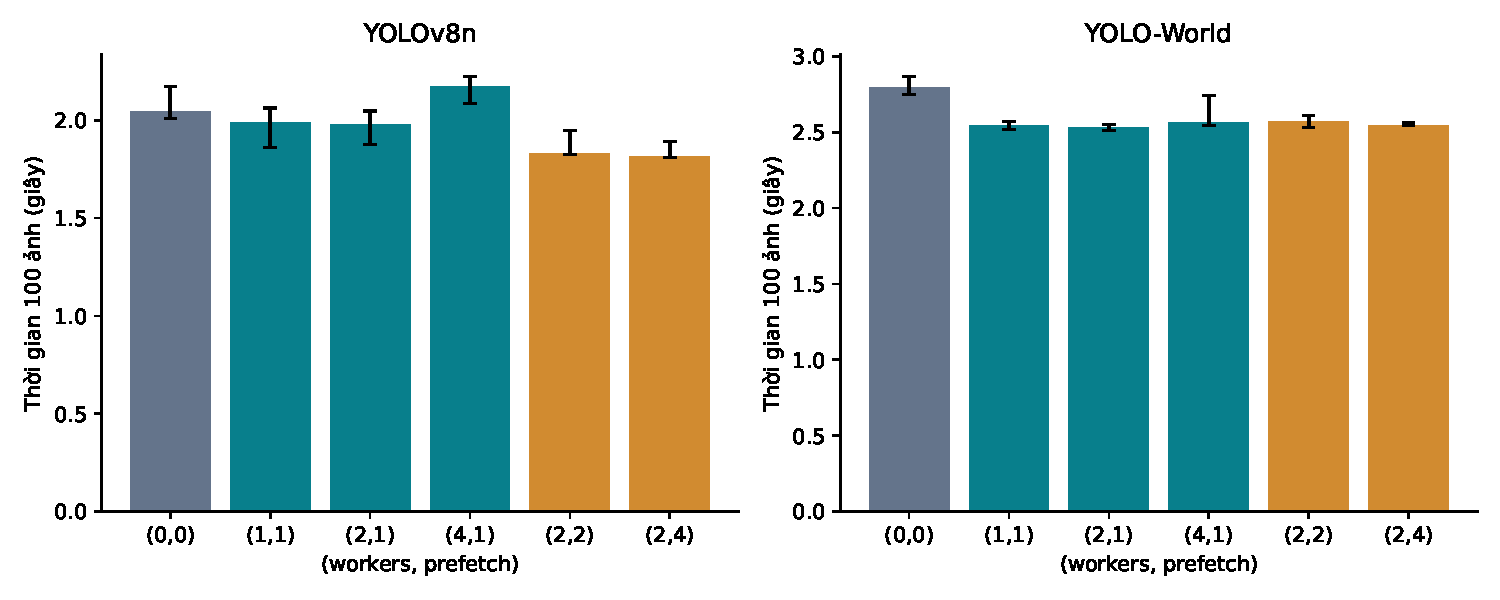
\includegraphics[width=\textwidth]{klygo/scheduling_comparison.pdf}
\caption{Thời gian xử lý theo cặp worker/prefetch; cột là trung vị, thanh sai số biểu diễn min--max của ba lượt}
\end{figure}
YOLOv8n: trung vị nhỏ nhất trong các cấu hình đã đo là (2,4) với 1.82 s; mặc định (1,1) là 1.99 s và tuần tự (0,0) là 2.05 s. Đây là mô tả phiên đo, không khẳng định cấu hình tối ưu trên mọi workload.

Sáu cấu hình YOLOv8n có 0/600 cặp frame vượt tiêu chí tương đương so với Raw, với cùng ngưỡng sai số như benchmark sáu mode.

YOLO-World: trung vị nhỏ nhất trong các cấu hình đã đo là (2,1) với 2.53 s; mặc định (1,1) là 2.54 s và tuần tự (0,0) là 2.80 s. Đây là mô tả phiên đo, không khẳng định cấu hình tối ưu trên mọi workload.

Sáu cấu hình YOLO-World có 0/600 cặp frame vượt tiêu chí tương đương so với Raw, với cùng ngưỡng sai số như benchmark sáu mode.

Chọn cấu hình sử dụng còn phụ thuộc độ trễ chấp nhận được và ngân sách RAM. Tăng worker/prefetch không có cam kết giảm thời gian đơn điệu; lợi ích chỉ xuất hiện khi nó giúp giải mã theo kịp mô hình, trong khi các chi phí đồng bộ và giữ pixel vẫn tồn tại. Phiên đo hữu hạn này chưa đánh giá nguồn video dài, batch lớn hay đọc dữ liệu qua mạng. Vì các cấu hình chưa được chạy theo thứ tự ngẫu nhiên cân bằng, kết quả cần được tái kiểm chứng trước khi dùng làm khuyến nghị triển khai chung.

